\apendice{Especificación de Requisitos}

\section{Introducción}
En este apartado, se van a explicar los requisitos tanto funcionales como no funcionales de la aplicación web realizada, así como los casos de uso y los actores intervienen en ellos.
\section{Objetivos generales}
El objetivo perseguido en este punto es el de implementar una aplicación web capaz de detectar el Parkinson que no requiera demasiados conocimientos para poder utilizarla.
\section{Catálogo de requisitos}
En esta sección, se detallan los requisitos funcionales y no funcionales de la aplicación web realizada.

\subsection{Requisitos funcionales}

\begin{itemize}
	\item \textbf{RF-1 Restricción de acceso a la aplicación:} para poder acceder al sistema, será necesario haberse dado de alta en él.
	\begin{itemize}
		\item \textbf{RF-1.1 Acceso:} los usuarios dados de alta podrán ingresar en la aplicación utilizando su nombre de usuario y su contraseña.
		\item \textbf{RF-1.2 Administración:} habrá un usuario administrador con más acceso que el resto.
	\end{itemize}
	\item \textbf{RF-2 Gestión de usuarios:} el administrador será el único usuario capaz de añadir, modificar y eliminar usuarios.
	\begin{itemize}
		\item \textbf{RF-2.1 Añadir usuario:} se podrá registrar un usuario en la aplicación.
		\item \textbf{RF-2.2 Modificar usuario:} se podrá modificar alguno de los datos de un usuario existente.
		\item \textbf{RF-2.3 Eliminar ususario:} se podrá eliminar un usuario de la aplicación.
	\end{itemize}
	\item \textbf{RF-3 Subida de datos al servidor:} se podrán subir ciertos datos importantes para detectar el Parkinson.
	\begin{itemize}
		\item \textbf{RF-3.1 Subida de vídeos:} se podrá subir un vídeo al servidor.
		\item \textbf{RF-3.2 Introducción de datos:} se podrá rellenar unos campos con información adicional.
	\end{itemize}
	\item \textbf{RF-4 Visualización del resultado:} se podrá ver si la persona del vídeo subido tiene Parkinson o no.
	\item \textbf{RF-5 Modificar modelo:} se podrá cambiar el modelo de predicción. 
\end{itemize}

\subsection{Requisitos no funcionales}
\begin{itemize}
	\item \textbf{RNF-1 Usabilidad:} la aplicación tendrá una interfaz amigable para que pueda ser usada sin dificultad.
	\item \textbf{RNF-2 Privacidad:} sólo se podrá acceder a la aplicación si el usuario está dado de alta.
	\item \textbf{RNF-3 Seguridad:} cada usuario dispondrá de una clave que estará encriptada para no ser interceptada por terceros.
	
	
\end{itemize}

\section{Especificación de requisitos}
En esta sección se detalla de forma profunda los casos de uso, qué actores participan en los casos de uso y los correspondientes diagramas.

\subsection{Actores}
Los actores que participan en la aplicación son:

\begin{itemize}
	\item \textbf{Administrador:} dispondrá de todas las funcionalidades con el fin de poder realizar una gestión en la aplicación.
	\item \textbf{Usuario:} podrá subir vídeos al servidor para ser procesados y que se identifique si el usuario tiene Parkinson.
\end{itemize}

\subsection{Diagramas de casos de uso}
Los diagramas de casos de uso por niveles, figuras \ref{fig:nivel_0} y \ref{fig:gestion_usuarios}, son los siguientes:

\begin{figure}[h]
	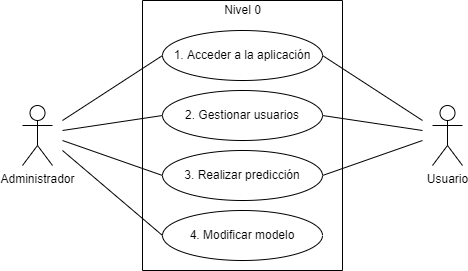
\includegraphics[width=1\textwidth]{nivel_0}
	\caption{Nivel 0 del diagrama de casos de uso.}
	\label{fig:nivel_0}
\end{figure}

\begin{figure}[h]
	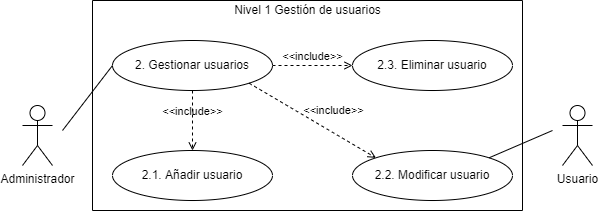
\includegraphics[width=1\textwidth]{gestion_usuarios}
	\caption{Nivel 1 Gestión de usuarios del diagrama de casos de uso.}
	\label{fig:gestion_usuarios}
\end{figure}

\subsection{Especificación de los casos de uso}
Las redacciones de los casos de uso de los diagramas anteriores, tablas \ref{tab:cu1}, \ref{tab:cu2}, \ref{tab:cu2_1}, \ref{tab:cu2_2}, \ref{tab:cu2_3}, \ref{tab:cu3} y \ref{tab:cu4} son las siguientes:

\begin{table}
	\begin{center}
		\begin{tabular}{| c | c | c |}
			\noalign{\hrule height 1.25pt}
			\rowcolor{gray!50}
			\multicolumn{3}{!{\vrule width 1.25pt} p{13.75cm} !{\vrule width 1.25pt}}{CU-1 Acceder a la aplicación} \\ \noalign{\hrule height 1.25pt}
			Dependencias & \multicolumn{2}{p{10cm} |}{
				\begin{itemize}
					\item RF-1 Restricción de acceso a la aplicación.
					\item RF-1.1 Acceso.
					\item RF-1.2 Administración.
				\end{itemize}} \\ \hline
			Actores & \multicolumn{2}{p{10cm} |}{Administrador y usuario} \\ \hline
			Precondición & \multicolumn{2}{p{10cm} |}{No hay ninguna sesión iniciada.} \\ \hline
			Descripción & \multicolumn{2}{p{10cm} |}{Se accede a la aplicación utilizando un nombre de usuario y una contraseña.} \\ \hline
			Secuencia normal & Paso & Acción \\ \cline{2-3}
			& 1 & \multicolumn{1}{p{8.75cm} |}{Se escribe el nombre de usuario y la contraseña para acceder.} \\ \cline{2-3}
			& 2 & \multicolumn{1}{p{8.75cm} |}{El servidor comprueba si es correcto y permite acceder al usuario.} \\ \hline
			Postcondición & \multicolumn{2}{p{10cm} |}{El usuario accede a la aplicación.} \\ \hline
			Excepciones & Paso & Acción \\ \cline{2-3}
			& 2 & \multicolumn{1}{p{8.75cm} |}{Si el nombre de usuario y/o la contraseña no son correctos no se accederá a la aplicación y se mostrará un error.} \\ \hline
			Comentarios & \multicolumn{2}{p{10cm} |}{Si el usuario no ha iniciado sesión sólo podrá acceder a esta ventana.} \\ \hline
		\end{tabular}
			\caption{Caso de uso 1: Acceder a la aplicación.}
			\label{tab:cu1}
	\end{center}
\end{table}

\begin{table}
	\begin{center}
		\begin{tabular}{| c | c | c |}
			\noalign{\hrule height 1.25pt}
			\rowcolor{gray!50}
			\multicolumn{3}{!{\vrule width 1.25pt} p{13.75cm} !{\vrule width 1.25pt}}{CU-2 Gestionar usuarios} \\ \noalign{\hrule height 1.25pt}
			Dependencias & \multicolumn{2}{p{10cm} |}{
				\begin{itemize}
					\item RF-2 Gestión de usuarios.
			\end{itemize}} \\ \hline
			Actores & \multicolumn{2}{p{10cm} |}{Administrador} \\ \hline
			Precondición & \multicolumn{2}{p{10cm} |}{Haber iniciado sesión con el usuario administrador.} \\ \hline
			Descripción & \multicolumn{2}{p{10cm} |}{Se muestran los usuarios registrados y las operaciones de añadir, modificar y eliminar.} \\ \hline
			Secuencia normal & Paso & Acción \\ \cline{2-3}
			& 1 & \multicolumn{1}{p{8.75cm} |}{Se accede a la ventana de gestión de usuarios.} \\ \hline
			Postcondición & \multicolumn{2}{p{10cm} |}{Se puede realizar la gestión de usuarios.} \\ \hline
			Excepciones & Paso & Acción \\ \cline{2-3}
			& 1 & \multicolumn{1}{p{8.75cm} |}{Si no se inicia sesión, el servidor redirigirá el acceso a la ventana de inicio de sesión.} \\ \hline
			& 1 & \multicolumn{1}{p{8.75cm} |}{Si el usuario no es el administrador, el servidor redirigirá el acceso a la ventana inicial.}  \\ \hline
		\end{tabular}
		\caption{Caso de uso 2: Gestionar usuarios.}
		\label{tab:cu2}
	\end{center}
\end{table}

\begin{table}
	\begin{center}
		\begin{tabular}{| c | c | c |}
			\noalign{\hrule height 1.25pt}
			\rowcolor{gray!50}
			\multicolumn{3}{!{\vrule width 1.25pt} p{13.75cm} !{\vrule width 1.25pt}}{CU-2.1 Añadir usuario} \\ \noalign{\hrule height 1.25pt}
			Dependencias & \multicolumn{2}{p{10cm} |}{
				\begin{itemize}
					\item RF-2.1 Añadir usuario.
			\end{itemize}} \\ \hline
			Actores & \multicolumn{2}{p{10cm} |}{Administrador} \\ \hline
			Precondición & \multicolumn{2}{p{10cm} |}{Haber iniciado sesión con el usuario administrador.} \\ \hline
			Descripción & \multicolumn{2}{p{10cm} |}{Se registra un nuevo usuario a la aplicación.} \\ \hline
			Secuencia normal & Paso & Acción \\ \cline{2-3}
			& 1 & \multicolumn{1}{p{8.75cm} |}{Se accede a la ventana de añadir usuario.} \\ \cline{2-3}
			& 2 & \multicolumn{1}{p{8.75cm} |}{Se rellenan los campos del nuevo usuario: nombre completo, nombre de usuario y contraseña.} \\ \cline{2-3}
			& 3 & \multicolumn{1}{p{8.75cm} |}{Se almacenan los datos.}\\ \hline
			Postcondición & \multicolumn{2}{p{10cm} |}{Se añade un nuevo usuario.} \\ \hline
			Excepciones & Paso & Acción \\ \cline{2-3}
			& 1 & \multicolumn{1}{p{8.75cm} |}{Si no se inicia sesión, el servidor redirigirá el acceso a la ventana de inicio de sesión.} \\ \hline
			& 1 & \multicolumn{1}{p{8.75cm} |}{Si el usuario no es el administrador, el servidor redirigirá el acceso a la ventana inicial.} \\ \cline{2-3}
			& 2 & \multicolumn{1}{p{8.75cm} |}{Si no se han rellenado todos los campos no se podrá añadir el usuario.} \\ \cline{2-3}
			& 2 & \multicolumn{1}{p{8.75cm} |}{Si el usuario existe no se podrá añadir el usuario.} \\ \hline
		\end{tabular}
		\caption{Caso de uso 2.1: Añadir usuario.}
		\label{tab:cu2_1}
	\end{center}
\end{table}

\begin{table}
	\begin{center}
		\begin{tabular}{| c | c | c |}
			\noalign{\hrule height 1.25pt}
			\rowcolor{gray!50}
			\multicolumn{3}{!{\vrule width 1.25pt} p{13.75cm} !{\vrule width 1.25pt}}{CU-2.2 Modificar usuario} \\ \noalign{\hrule height 1.25pt}
			Dependencias & \multicolumn{2}{p{10cm} |}{
				\begin{itemize}
					\item RF-2.2 Modificar usuario.
			\end{itemize}} \\ \hline
			Actores & \multicolumn{2}{p{10cm} |}{Administrador} \\ \hline
			Precondición & \multicolumn{2}{p{10cm} |}{Haber iniciado sesión con el usuario administrador.} \\ \hline
			Descripción & \multicolumn{2}{p{10cm} |}{Se modifica un usuario existente de la aplicación.} \\ \hline
			Secuencia normal & Paso & Acción \\ \cline{2-3}
			& 1 & \multicolumn{1}{p{8.75cm} |}{Se accede a la ventana de modificar usuario.} \\ \cline{2-3}
			& 2 & \multicolumn{1}{p{8.75cm} |}{Se modifican los campos del usuario: nombre completo, nombre de usuario y contraseña.} \\ \cline{2-3}
			& 3 & \multicolumn{1}{p{8.75cm} |}{Se almacenan los datos.}\\ \hline
			Postcondición & \multicolumn{2}{p{10cm} |}{Se modifica el usuario existente.} \\ \hline
			& 1 & \multicolumn{1}{p{8.75cm} |}{Si no se inicia sesión, el servidor redirigirá el acceso a la ventana de inicio de sesión.} \\ \hline
			Excepciones & Paso & Acción \\ \cline{2-3}
			& 1 & \multicolumn{1}{p{8.75cm} |}{Si el usuario no es el administrador, el servidor redirigirá el acceso a la ventana inicial.} \\ \cline{2-3}
			& 2 & \multicolumn{1}{p{8.75cm} |}{Si no se han rellenado todos los campos no se podrá modificar el usuario.} \\ \cline{2-3}
			& 2 & \multicolumn{1}{p{8.75cm} |}{Si el usuario existe no se podrá modificar el usuario.} \\ \hline
		\end{tabular}
		\caption{Caso de uso 2.2: Modificar usuario.}
		\label{tab:cu2_2}
	\end{center}
\end{table}

\begin{table}
	\begin{center}
		\begin{tabular}{| c | c | c |}
			\noalign{\hrule height 1.25pt}
			\rowcolor{gray!50}
			\multicolumn{3}{!{\vrule width 1.25pt} p{13.75cm} !{\vrule width 1.25pt}}{CU-2.3 Eliminar usuario} \\ \noalign{\hrule height 1.25pt}
			Dependencias & \multicolumn{2}{p{10cm} |}{
				\begin{itemize}
					\item RF-2.3 Eliminar usuario.
			\end{itemize}} \\ \hline
			Actores & \multicolumn{2}{p{10cm} |}{Administrador} \\ \hline
			Precondición & \multicolumn{2}{p{10cm} |}{Haber iniciado sesión con el usuario administrador.} \\ \hline
			Descripción & \multicolumn{2}{p{10cm} |}{Se elimina un usuario existente de la aplicación.} \\ \hline
			Secuencia normal & Paso & Acción \\ \cline{2-3}
			& 1 & \multicolumn{1}{p{8.75cm} |}{Se selecciona el usuario que se desea eliminar} \\ \cline{2-3}
			& 2 & \multicolumn{1}{p{8.75cm} |}{Se confirma el usuario que se desea eliminar.} \\ \hline
			Postcondición & \multicolumn{2}{p{10cm} |}{Se elimina el usuario.} \\ \hline
			Excepciones & Paso & Acción \\ \cline{2-3}
			& 1 & \multicolumn{1}{p{8.75cm} |}{Si no se inicia sesión, el servidor redirigirá el acceso a la ventana de inicio de sesión.} \\ \hline
			& 1 & \multicolumn{1}{p{8.75cm} |}{Si el usuario no es el administrador, el servidor redirigirá el acceso a la ventana inicial.} \\ \hline
		\end{tabular}
		\caption{Caso de uso 2.3: Eliminar usuario.}
		\label{tab:cu2_3}
	\end{center}
\end{table}

\begin{table}
	\begin{center}
		\begin{tabular}{| c | c | c |}
			\noalign{\hrule height 1.25pt}
			\rowcolor{gray!50}
			\multicolumn{3}{!{\vrule width 1.25pt} p{13.75cm} !{\vrule width 1.25pt}}{CU-3 Realizar predicción} \\ \noalign{\hrule height 1.25pt}
			Dependencias & \multicolumn{2}{p{10cm} |}{
				\begin{itemize}
					\item RF-3 Subida de datos al servidor.
					\item RF-3.1 Subida de vídeos.
					\item RF-3.2 Introducción de datos.
					\item RF-4 Visualización del resultado.
			\end{itemize}} \\ \hline
			Actores & \multicolumn{2}{p{10cm} |}{Administrador y usuario} \\ \hline
			Precondición & \multicolumn{2}{p{10cm} |}{Haber iniciado sesión.} \\ \hline
			Descripción & \multicolumn{2}{p{10cm} |}{Se suben los datos para realizar la predicción.} \\ \hline
			Secuencia normal & Paso & Acción \\ \cline{2-3}
			& 1 & \multicolumn{1}{p{8.75cm} |}{Se accede a la ventana.} \\ \cline{2-3}
			& 2 & \multicolumn{1}{p{8.75cm} |}{El usuario sube el vídeo y los datos al servidor.} \\ \cline{2-3} 
			& 3 & \multicolumn{1}{p{8.75cm} |}{Se muestra el resultado de la predicción.} \\ \hline
			Postcondición & \multicolumn{2}{p{10cm} |}{El usuario obtiene una predicción.} \\ \hline
			Excepciones & Paso & Acción \\ \cline{2-3}
			& 1 & \multicolumn{1}{p{8.75cm} |}{Si no se inicia sesión, el servidor redirigirá el acceso a la ventana de inicio de sesión.} \\ \hline
		\end{tabular}
		\caption{Caso de uso 3: Realizar predicción.}
		\label{tab:cu3}
	\end{center}
\end{table}

\begin{table}
	\begin{center}
		\begin{tabular}{| c | c | c |}
			\noalign{\hrule height 1.25pt}
			\rowcolor{gray!50}
			\multicolumn{3}{!{\vrule width 1.25pt} p{13.75cm} !{\vrule width 1.25pt}}{CU-4 Modificar modelo} \\ \noalign{\hrule height 1.25pt}
			Dependencias & \multicolumn{2}{p{10cm} |}{
				\begin{itemize}
					\item RF-5 Modificar modelo.
			\end{itemize}} \\ \hline
			Actores & \multicolumn{2}{p{10cm} |}{Administrador} \\ \hline
			Precondición & \multicolumn{2}{p{10cm} |}{Haber iniciado sesión con el usuario administrador.} \\ \hline
			Descripción & \multicolumn{2}{p{10cm} |}{Se modifica el modelo de predicción.} \\ \hline
			Secuencia normal & Paso & Acción \\ \cline{2-3}
			& 1 & \multicolumn{1}{p{8.75cm} |}{Se accede a la ventana.} \\ \cline{2-3}
			& 2 & \multicolumn{1}{p{8.75cm} |}{Se sube el nuevo modelo.} \\ \hline
			Postcondición & \multicolumn{2}{p{10cm} |}{Las predicciones se harán con el nuevo modelo.} \\ \hline
			Excepciones & Paso & Acción \\ \cline{2-3}
			& 1 & \multicolumn{1}{p{8.75cm} |}{Si no se inicia sesión, el servidor redirigirá el acceso a la ventana de inicio de sesión.} \\ \cline{2-3}
			& 1 & \multicolumn{1}{p{8.75cm} |}{Si el usuario no es el administrador, el servidor redirigirá el acceso a la ventana inicial.} \\ \hline
		\end{tabular}
		\caption{Caso de uso 4: Modificar modelo.}
		\label{tab:cu4}
	\end{center}
\end{table}
